
\chapter{State of the Art}

\section{Optimization}

\subsection{Basic Concepts}

Before starting to present the different categories of optimization and some related existing methods, we would like to take some time defining what exactly optimization is. In the more general way, optimizing is \emph{trying to find the best element among an element set} (when finding this best element is not trivial, we can rightfully talk of \emph{solving an optimization problem). }This somewhat simple definition implies in fact quite a lot.

First of all it implies we have a defined set of element to choose from. As we will see, the topology of the set is in fact of the utmost importance for solving the problem. This set of element is often named the \emph{search space}, \emph{solution space} or \emph{domain}. In {}``simple'' optimization problems, the search space can be simply defined by a set of elements (for example \{a,b,c\} or \ensuremath{\mathbb{R}}) associated with a set of \emph{constraints}. For large problems, the search space can be defined by calculus-heavy equations, empirical models, complex algorithms ... or even a mix of all of the above.

Since we want to find the best element of this solution space, we have to determine what make an element better than another. Usually, the possible solutions are compared through a specific function called the \emph{objective function}. Some alternate names are \emph{criterion} or \emph{cost function}. The best element would be the one for which the objective function returns a minimal (or alternatively, maximal\footnote{Obviously we sometimes want to find the \emph{maximal} value which is solution of a problem, however minimizing f(x) is equivalent to maximizing (-f(x)). So maximization problems can be expressed as minimization problems, and vice-versa. Traditionally, optimization problems are often expressed in the terms of finding a \emph{minimal} value since the two possibilities are equivalents.}) value. It should be noted that it is possible for a problem to admit several equivalent solutions in regard of the objective function.

The least obvious keyword here is \emph{try}. When the search space is very large, or its topology is complicated, it can be really long or difficult to find the best solution and, more important, to be sure that the solution is the best. In fact, in these problems, the only way to find the best solution with certainty is an exhaustive exploration of the search space. Since it can be very costly in terms
of time and calculation, instead of finding the best solution, we settle for a solution which is {}``good enough'', for example because this solution is the best for a subpart of the search space. The best solution is called the \emph{global optimum}, while a {}``good enough'' solution is called a \emph{local optimum}. In a similar fashion, methods which try to find the global solution are said to be \emph{global optimization methods}, where methods which search for local optimum are said to be \emph{local optimization methods}.

\begin{figure}
\centering
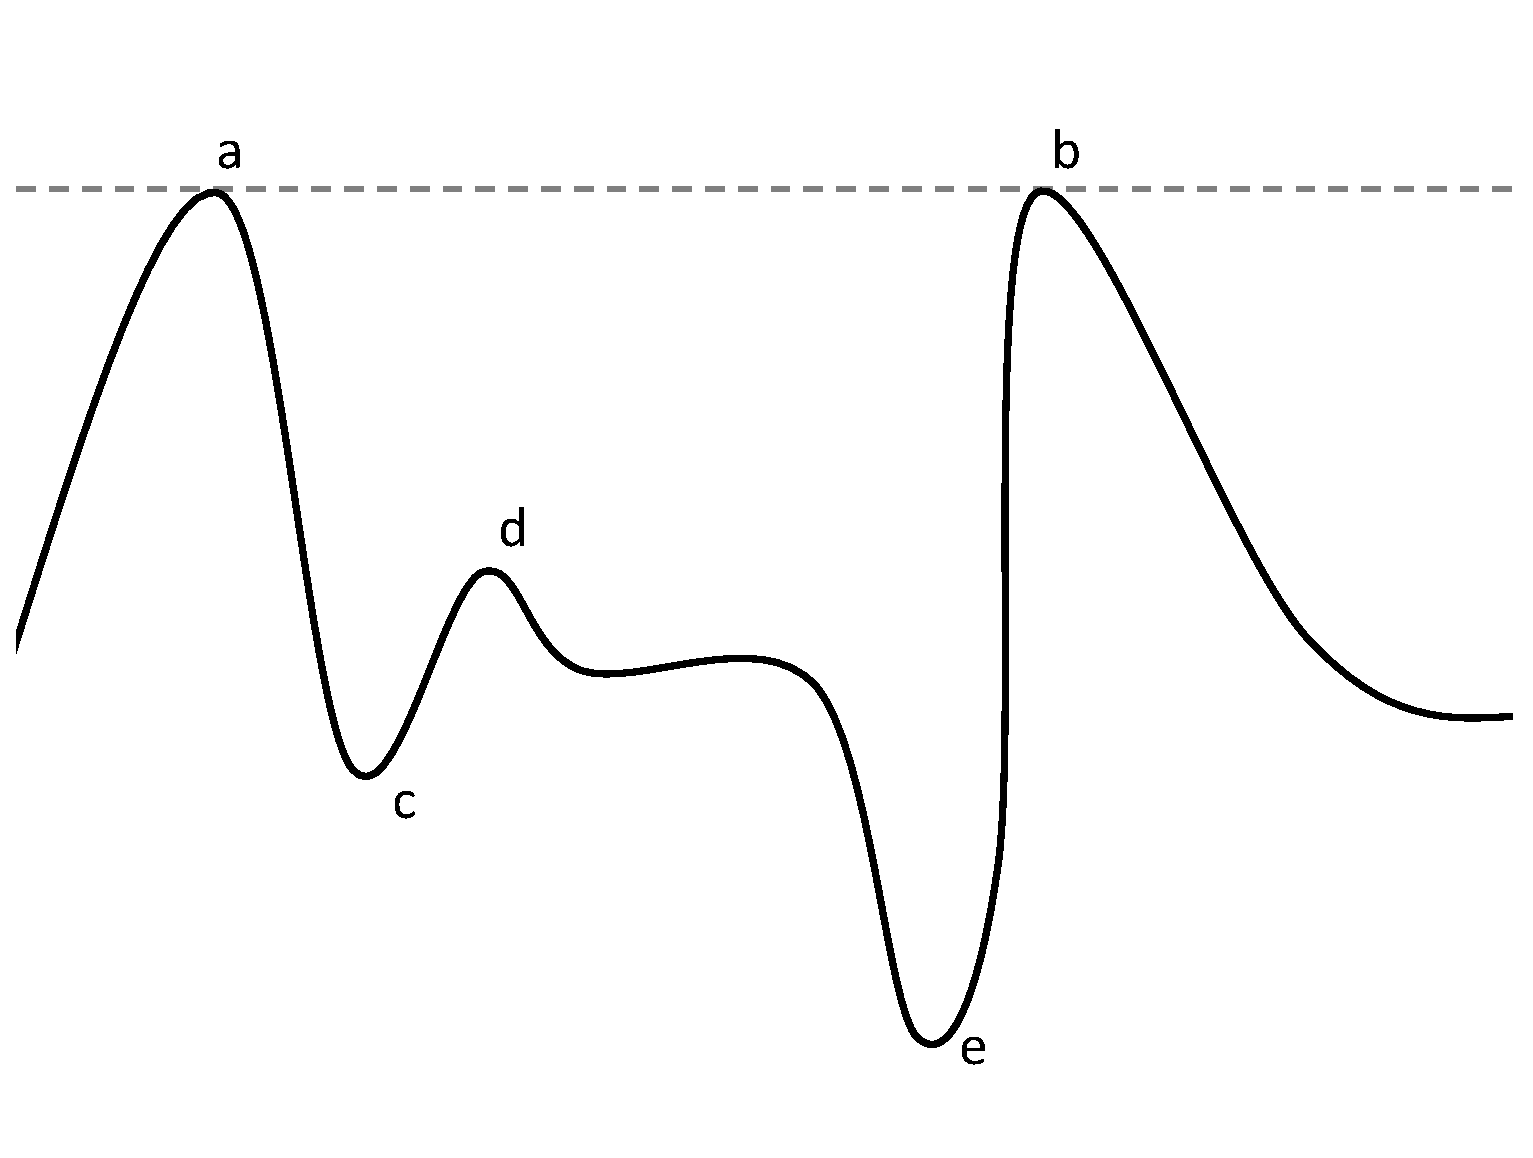
\includegraphics[width=0.6\paperwidth]{searchSpace}
\caption{Examples of local and global optimums.}
\label{localAndGlobalOptims}
\end{figure}


In \ref{localAndGlobalOptims}, we can see different examples of global and local optimums. The points labeled \emph{a} and \emph{b} are both global maximums, as they have the same value. The points
\emph{c} and \emph{d} are respectively local minimum and maximum, while \emph{e} is the global minimum.

A formal definition of the most simple and generic optimization problem would be:

\begin{equation}
min\, f(x)\, s.t.\,(x\in X)
\end{equation}

Where \emph{X} is our search space and \emph{f(x)} the objective function we want to minimize. 

\subsubsection{No Free Lunch Theorem}

\subsubsection{Combinatorial Optimization}

\subsection{Numerical Optimization}
\subsubsection{Linear Programming}
\subsubsection{Quadratic Programming}
\subsection{Nonlinear Programming}

\subsection{Multi-Objective Optimization}

Multi-objective optimization (also called multi-criteria optimization), or MOO, departs significantly from previous categories of optimization in the fact that you have to consider multiple objective functions instead of one. A main aspect of MOO is the way to conciliate these objectives, which are usually contradictory.
An example of real-world everyday MOO problem could be choosing the mean of transportation for a travel, trying to find a balance between speed and cost. Airplane is the fastest way of transportation, but is expensive. While car is slower, it is cheaper. Train is slower than plane, more expensive than car, but can preferred as the best compromise. There still, however, are solutions which are strictly worse than others (in our example, renting an helicopter would probably be both more expensive and slower than buying a seat on a commercial airplane).
From this example, we can see that, for a MOO problem, there rarely is a clear-cut "best" solution. And, more importantly, that even some solutions which are not optimum for \emph{any} of the objectives can be deemed satisfying. 


[[FORMULATION OF A MOO PROBLEM]]

We will now see which strategies have been proposed to deal with such a type of problem.

\subsubsection{Objectives Aggregation}

The first approach is to transform the MOO problem back to a mono-objective optimization problem, by aggregating the different objectives into one.

[[Different strategies : pondered mean, goal programming, min-max -> See thesis JB Welcomme for ref]]

Whatever the chosen aggregation strategy will be, this approach presents severe limitations. 

\subsubsection{Pareto Dominance}

\subsubsection{\emph{A priory} versus \emph{a posteriori} approaches}

\subsection{Multidisciplinary Optimization}

\subsection{Optimization under Uncertainties}

\subsection{Optimization in Dynamic Environments}

\subsubsection{Genetic Algorithms}


\end{document}
